\documentclass{beamer}
\usepackage{bm,multirow}%,transparent}

\definecolor{myblue}{rgb}{0.05,0.32,0.63}
\everymath{\color{myblue}}

\title{\vskip5mm On modelling ballistic gelatine by smoothed particle hydrodynamics (SPH)}
\author{\vskip-5mm Lud\v{e}k Hyn\v{c}\'{\i}k}
\institute{New Technologies - Research Centre \\ University of West Bohemia \\ Czech Republic}
\date{\scriptsize 9$^\text{th}$ International Conference on Mechanics and Materials in Design \\ Funchal (Portugal) 26 - 30 June 2022}

\usepackage{tikz}
%\titlegraphic{ 
\logo{ 
\begin{tikzpicture}[overlay,remember picture];
\node[left=0.5cm] at (current page.32){\includegraphics[width=3cm]{Figures/logo_NTC}};
\end{tikzpicture}
}

\begin{document}

%%%%%%%%%%%%%%%%%%%%%%%%%%%%%%%%%%%%%%%%%%%%%%%%%%%%%%
\begin{frame}
\titlepage
\begin{tikzpicture}[overlay,remember picture];
\node[left=6cm] at (current page.32){
\includegraphics[width=6cm]{Figures/logo_SF}};
\end{tikzpicture}
\end{frame}

%%%%%%%%%%%%%%%%%%%%%%%%%%%%%%%%%%%%%%%%%%%%%%%%%%%%%%
\begin{frame}
\frametitle{Content}
\tableofcontents
\end{frame}

%%%%%%%%%%%%%%%%%%%%%%%%%%%%%%%%%%%%%%%%%%%%%%%%%%%%%%
\section{Introduction}

%%%%%%%%%%%%%%%%%%%%%%%%%%%%%%%%%%%%%%%%%%%%%%%%%%%%%%
\subsection{Motivation}

\begin{frame}
\frametitle{Introduction}
\begin{itemize}
\item Penetrating ballistic impact \\ for estimating consequences \\ and severity of gunshot wounds
\item Ethics motivates for using \\ substituting matter \\ and numerical modelling
\item Ballistic gelatine correlated well \\ to human muscle tissue
\item Smoothed particle hydrodynamics
\begin{itemize}
\item Ballistic gelatine highly sensitive to strain rate and temperature
\item Behaving as shear thickening fluid at high shear rates
\item Large deformations and material discontinuities
\end{itemize}
\item Numerical modelling of ballistic gelatine \\ for future use in virtual testing
\end{itemize}
\begin{tikzpicture}[overlay,remember picture];
\node[left=1cm] at (current page.10){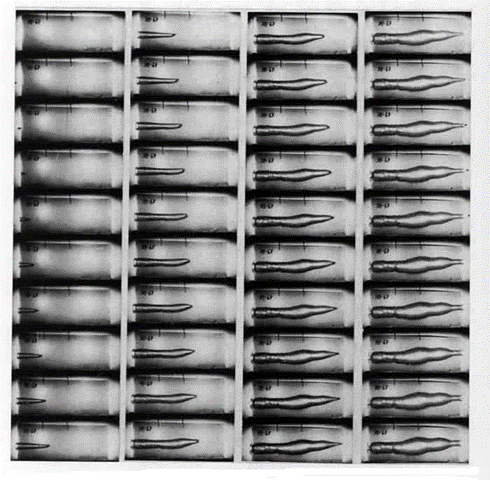
\includegraphics[width=4cm]{Figures/canal}};
\end{tikzpicture}
\end{frame}

%%%%%%%%%%%%%%%%%%%%%%%%%%%%%%%%%%%%%%%%%%%%%%%%%%%%%%
\section{Smoothed particle hydrodynamics}

\subsection{Basic theory of SPH}
\begin{frame}
\frametitle{Smoothed particle hydrodynamics}
\begin{itemize}
\item Mainly for astrophysical problems
\item Highly deformable solids
\item Considerably moving matter and boundaries
\item Conservation laws transformed into integral equations \\ by kernel function $w\left({\bm r}, h\right)$ with $\lim\limits_{h\rightarrow 0}w\left({\bm r}, h\right)=\delta\left({\bm r}\right)$
\item $w$ $\sim$ weighting function defining how much of each field variable contributes to field variable at given point in space \\
\vskip3mm
$\langle A\left({\bm r}\right)\rangle=\int\limits_V A\left({\bm r}^\prime\right)w\left({\bm r} - {\bm r}^\prime, h\right)d{\bm r}^\prime$ \\
$\langle A\left({\bm r}\right)\rangle=\sum\limits_{j=1}^{N}\frac{m_j}{\rho_j\left({\bm r}_j\right)}A\left({\bm r}_j\right)w\left({\bm r} - {\bm r}_j, h\right)$ \\
$\langle\nabla_r  A\left({\bm r}\right)\rangle=\sum\limits_{j=1}^{N}\frac{m_j}{\rho_j\left({\bm r}_j\right)}A\left({\bm r}_j\right)\nabla_r w\left({\bm r} - {\bm r}_j, h\right)$
\end{itemize}
\end{frame}

\begin{frame}
\frametitle{Driving equations}
\begin{itemize}
\item Equation of motion $\frac{d{\bm v}_i}{dt}=-\sum\limits_{j=1}^{N}m_j\left(\frac{p_j}{\rho_j^2}+\frac{p_i}{\rho_i^2}+\Pi_{ij}\right)\nabla_r w_{ij}$
\item Continuity equation $\frac{d\rho_i}{dt}=\sum\limits_{j=1}^{N}m_j\left({\bm v}_i-{\bm v}_j\right)\nabla_r w_{ij}$
\item Equation of conserving energy $\frac{du_i}{dt}=\sum\limits_{j=1}^{N}m_j\frac{p_j}{\rho_j^2}\left({\bm v}_i-{\bm v}_j\right)\nabla_r w_{ij}$
\item Artificial viscosity $\Pi_{ij}=\frac{1}{\rho_{ij}\left(-\alpha\mu_{ij}c_{ij}+\beta\mu_{ij}^2\right)}$, $A_{ij}=\frac{A_i-A_j}{2}$
\item Finding nearest particles contributing \\ to physical value of particular particle
\item Optimised nearest neighbour search
\end{itemize}
\end{frame}

\subsection{Viscous and incompressible matter}
\begin{frame}
\frametitle{Viscous and incompressible matter}
\begin{itemize}
\item Second derivative challenging
\item Run in quasi-incompressible limit \\
$p=K\left[\left(\frac{\rho}{\rho_0}\right)^\gamma-1\right]$ \\
$K=\frac{c^2\rho_0}{\gamma}$, $\gamma=7$
\item $K$ takes into account density fluctuations \\ under 1\% for weakly compressible fluid
\item For maximum flow speed $v$ $\frac{\delta p}{\rho_0}=\frac{v^2}{c^2}=M^2$
\end{itemize}
\end{frame}

\subsection{High-speed loading}
\begin{frame}
\frametitle{High-speed loading}
\begin{itemize}
\item Polynomial Mie-Gr\"uneisen equation of state
$p=\left\{\begin{matrix}
\sum\limits_{k=0}^3 C_k\eta^k+\left(C_4+C_5\eta\right)E_n\quad\forall\eta\ge 0\\
C_0+C_1\eta\quad\forall\eta<0
\end{matrix}\right.$ \\
$\eta=\frac{\rho}{\rho_0}-1$
\end{itemize}
\end{frame}

\subsection{Modelling ballistic gelatine}
\begin{frame}
\frametitle{Modelling ballistic gelatine}
\begin{itemize}
\item Hydrodynamic material
\item Highly viscous matter $\mu\sim 10\,m\cdot Pa\cdot s$ \\ for quasi-static loading
\item Dynamic viscosity $\mu\sim1000\times$ higher
\item Small cylinder sample \\ $h=d=6.35\,mm$
\end{itemize}
\end{frame}

\subsection{Numerical model setup}
\begin{frame}
\frametitle{Numerical model setup}
\begin{columns}
\column{0.5\textwidth}
\begin{itemize}
\item Symmetry in 2 planes
\item Uniform particle spacing $\Delta = 0.254\,mm$
\item 3025 particles in 3D
\item Frictionless contact between domain and plates
\item Pre-locating neighbouring particles
\item Static $\dot\epsilon=0.0\, s^{-1}$
\item Dynamic $\dot\epsilon=1000\,s^{-1}$
\end{itemize}
\column{0.5\textwidth}
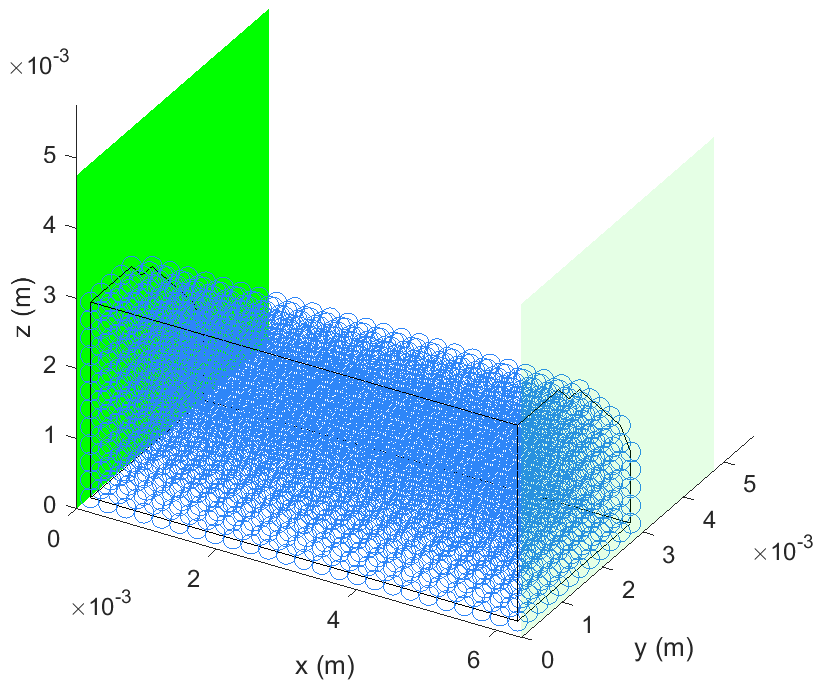
\includegraphics[width=6cm]{Figures/reference.png}
\end{columns}
\end{frame}

%%%%%%%%%%%%%%%%%%%%%%%%%%%%%%%%%%%%%%%%%%%%%%%%%%%%%%
\section{Results}
\subsection{Comparison to experimental data}
\begin{frame}
\frametitle{Results}
\begin{itemize}
\item Agreement to experimental data until $\epsilon=0.5$ \\ for both quasi-static and dynamic loadings
\begin{center}\includegraphics[width=4cm]{Figures/static_101.png}
\quad
\includegraphics[width=4cm]{Figures/dynamic_101.png}
\end{center}
\item Obvious non-uniform deformation
\end{itemize}
\end{frame}

%%%%%%%%%%%%%%%%%%%%%%%%%%%%%%%%%%%%%%%%%%%%%%%%%%%%%%
\section{Conclusion}
\subsection{Acknowledgements}
\begin{frame}
\frametitle{Conclusion}
\begin{itemize}
\item SPH implemented for ballistic gelatine numerical model
\item Generic material properties of ballistic gelatine
\item Numerical simulations verified the material model 
\begin{itemize}
\item Quasi-static compression
\item Dynamic compressions
\end{itemize}
\end{itemize}
\vskip5mm
{\small\color{myblue}This research was funded by the European Regional Development Fund-Project "Application of modern technologies in medicine and industry" (grant number CZ.02.1.01/0.0/0.0/17\_048/0007280).}
\begin{tikzpicture}[overlay,remember picture];
\node[left=3cm] at (current page.-30){
\includegraphics[width=6cm]{Figures/logo_SF}};
\end{tikzpicture}
\end{frame}

\end{document}
